\documentclass[11pt,a4paper]{article}
\usepackage[a4paper,left=1in, right=1in, top=1.5in, bottom=1.2in]{geometry}
\usepackage[latin1]{inputenc}
\usepackage{amsmath}
\usepackage{amsfonts}
\usepackage{amssymb}
\usepackage{graphicx}
\usepackage{cite}
\usepackage{enumitem}
%\usepackage{wasysym}
\usepackage[usenames,dvipsnames]{color}
\usepackage{tikz}
\usepackage{gantt}
\usepackage{caption}
\usepackage{enumitem}
\usepackage{comment}
\usepackage{textcomp}
%\excludecomment{thebibliography}


\usepackage{fancyhdr}
\setlength{\headheight}{0.4in}
\pagestyle{fancy}
\lhead{\textsc{{\large Transitions to Renewable Energy: \\
Modeling it from the Bottom-up and the Top-down
 }}}
\chead{}
\rhead{}

\lfoot{\textsc{Project Description}}
\cfoot{\textsc{Haney, Carbajales-Dale, Heun}}
\rfoot{\thepage}

\renewcommand{\headrulewidth}{0.4pt}
\renewcommand{\footrulewidth}{0.4pt}



\begin{document}


%\maketitle



%\maketitle

%\begin{itemize}
%	\item 	clear statement of the work to be undertaken 
%	\item 	objectives for the period of the proposed work and expected significance 
%	\item 	relation to longer-term goals of the PI's project 
%	\item	relation to the present state of knowledge in the field, 
%	\item	relation to work in progress by the PI under other support and to work in progress elsewhere
%	\item	outline the general plan of work, including:
%	\begin{itemize}
%		\item	broad design of activities to be undertaken,
%		\item	clear description of experimental methods and procedures. 
%	\end{itemize}
%	\item Proposers should address 
%	\begin{itemize}
%		\item	what they want to do, 
%		\item	why they want to do it, 
%		\item	how they plan to do it, 
%		\item	how they will know if they succeed, and 
%		\item	what benefits could accrue if the project is successful. 
%	\end{itemize}
%	\item	must contain, as a separate section within the narrative, a discussion of the broader impacts of the proposed activities.
%\end{itemize}	
%
%\part{What we want to do}

%Page 1, First sentence --- “The objective of this proposal is to…..”
%Page 1, first paragraph: Overview of the project concisely identifying knowledge gaps (page 5 below) and how great you/your team is with the clever ways you will solve the knowledge gaps (page 6-7 below) 
%Page 1-3: Background information giving the state of the art in your science/engineering field. Be sure to include your own contributions. 
%Page 4-5: knowledge gaps: Identify what is wrong with the state of the art. Explain what you will cover in this proposal and what you won’t cover (and why). 
%Page 5-7: Clearly and concisely discuss how you are going to address the knowledge gaps with a series of specific hypotheses and objectives. A table linking hypotheses, objectives, and tasks is quite effective (Write this section first)
%Page 7-13: Detailed task descriptions. Show how tasks are interrelated. 
%Page 14: Listing of personnel and qualifications to show reviewers that you can do the work proposed above
%Page 15: Impact, what “product” will you deliver to the funding agency. 

\begin{table}
\begin{tabular}{lp{12cm}}
	\textsc{PI} & \textsc{Dr. Becky Haney, Economics, Calvin College, Grand Rapids, MI 49546}	\\
	\textsc{co-PI} & \textsc{Dr. Michael Carbajales-Dale, Environmental Engineering \& Earth Sciences, Clemson University, Clemson SC 29634} \\
	\textsc{co-PI} & \textsc{Dr. Matthew Heun, Engineering, Calvin College, Grand Rapids, MI 49546} \\
\end{tabular}
\end{table}
\section{Introduction}

The objective of this proposal is to test the hypothesis that 
interacting agents are unable to collectively manage 
a transition from non-renewable to renewable resources 
to avoid negative impacts of resource depletion. 
Since Hardin's seminal paper, ``The tragedy of the commons'',
it has been understood that individuals acting purely out of self-interest
are likely to degrade commonly-owned resources~\cite{Hardin1968}.
This finding is in direct tension with the notion of
``the invisible hand'' of the market,
promoted within economics~\cite{Smith1776}.
The depletion of stock-based resources
(especially fossil-based energy resources
and their associated climate change impacts),
necessitates a transition to flow-based, renewable resources
and the closing of material pathways within our economies.
Policy planning is currently guided by integrated assessment models (IAM).
Such models typically represent resource utilization and infrastructure investment decisions,
purely in terms of financial transactions controlled by a centralized authority.
Unfortunately, such a representation fails to account either for
(i) the physical resources (energy and materials) 
to build out the required infrastructure, and
(ii) the multiplicity of individual decision-makers that comprise 
global resource supply and investment networks.
The Energy-Economy-Environment (E$^3$) Systems Analysis group
at Clemson has expertise both in 
material and energy requirements for critical infrastructure 
and in modeling multiple-actor interactions.
In developing an agent-based approach to test our hypothesis,
we will be able to generate better models and recommendations 
for policy and decision support.

Figure~\ref{fig:CNH_Schema}

\begin{figure}
\centering\
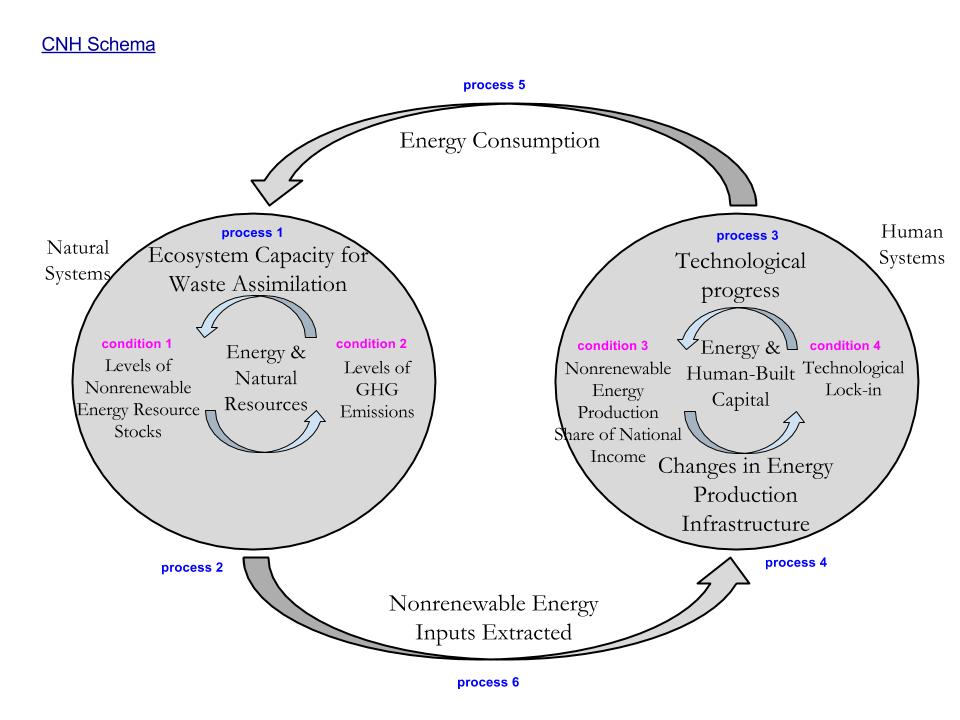
\includegraphics[width=\linewidth]{CNH_Schema.jpg}
\caption[CNH Schema]{CNH Schema for Energy Transitions.}
\label{fig:CNH_Schema}
\end{figure}

%\part{Why we want to do it}

\section{Background and motivation}
\label{sec:back}

The modern energy-economy-environment (E3) system is incredibly complex.
Dynamics within the natural system impact and are themselves impacted by
increasingly complex dynamics within the human-built system.
Over the course of the 21$^{st}$ Century, 
increasing social stressors, including
global population,
raising living standards
improving access to modern energy infrastructure,
will place strong pressure on the capacity of the biosphere
to support such demands,
especially in light of biophysical stressors,
such as climate change,
resource depletion, and
ecosystem degradation~\cite{IPCC2014}.
A transition is required within industrial society,
to modes of operation that
(i) use renewable resources (such as forest products) 
at rates lower than their rate of regeneration;
(ii) emit wastes (such as carbon dioxide) 
at rates lower than their assimilation by environmental systems; and
(iii) reduce the use of non-renewable resources (such as crude oil) 
to rates at which renewable substitutes can be deployed~\cite{Goodland1996, G-R1971}.

Models and tools for policy planning and decision support
overwhelmingly cast interactions within the economy
purely in terms of flows of financial data%~(for example MESSAGE-MACRO~\cite{Klaassen2007}).
Integrated assessment models (IAM)
represent the economy using a number of separate modules, 
including the energy sector 
(such as MESSAGE~\cite{Messner2000} or MarkAL~\cite{Seebregts2002}), 
and the macro-economy,
modeled via computable general equilibrium model
(such as GEMINI-E3~\cite{Bernard2008} or E3MG~\cite{Kohler2006}). 
Demand for energy depends on various factors including 
population, 
gross domestic product (GDP, disaggregated by sectors), 
and sectoral energy intensity. 

The core of the energy sector module is typically 
some reference energy system where demand for 
energy services (transport, space heat, light, etc.) 
is met from a variety of energy resources (coal, gas, etc.) 
by linking appropriate energy conversion technologies, 
each with an associated financial cost, 
determined by the user. 
The module seeks to meet an objective function 
wherein energy demand is met at the minimum overall system cost. 
The only input required by the energy sector 
are sufficient monetary flows, 
not the necessary energy and materials required for 
infrastructure investment or operation.

Whilst financial flows represent an important aspect of modern society,
it is crucial that we also gain a better understanding of 
the physical structure of our economies,
for it is in the exchange of energy and materials,
that human societies interface with the natural systems
within which they are embedded and upon which 
they are entirely dependent~\cite{Heun2015, Dale2012a}.
The field of net energy analysis (NEA)
seeks to understand and characterize the 
energy and materials that society must invest
in order to transform primary energy resources into economic services,
at a variety of scales ranging from individual solar photovoltaic (PV) panels 
to whole industries or even whole economies.
%A number of researchers have have characterized economic industries or sectors
%(particularly the energy sector)
%and even the whole economy
%in terms of flows of physical materials and/or energy. %~\cite{Wiedmann2015, Dale2013, Dale2012b, Slesser1992, Cleveland1984}.
A number of models have been developed 
which trace physical flows of energy (and materials) 
through the economy to explore 
the economic implications of resource constraints. 
Undoubtedly the most famous of this type of 
physical resource model is the World3 model from 
the `Limits to Growth' report by the Club of Rome~\cite{Meadows1972}. 
Other models include the System, Time, Energy \& Resources (STER) model~\cite{Hounam1979}; 
the Dynamic Energy model to explore the New Zealand  and global  economies~\cite{Baines1983, Bodger1989}; 
and the Energy and Capital Creation Options (ECCO) model~\cite{Slesser1992}.

To build on this work, the PI created 
the Global Energy Model using a Biophysical Approach (GEMBA) 
to integrate pertinent data from the field of NEA 
to enable a model that optimized for energetic costs involved in 
manufacturing and operating the infrastructure of the energy sector, 
in an analogous manner to the financial cost optimization 
in the traditional economic modeling approach. 
The model includes feedback between the energy sector 
and the rest of the economy. 
Subsequent work by the PI has utilized data from LCA 
and focused in greater detail on specific energy technologies 
including solar photovoltaic (PV) , wind and storage . 

Correspondingly,
policy planning models also cast (`top-down') investment decisions 
within the economy as undertaken via a central agency,
with perfect knowledge and perfect foresight, 
or with some randomly generated, 
exogenously defined level of `uncertainty'~\cite{Hu2010}.
The structure of such models
is implicitly founded upon the existence both 
an equilibrium state for the economy
and an optimal pathway to reach that state~\cite{}.

In rejection to this perspective,
researchers in non-equilibrium and complexity economics
seek to understand the economy as a 
thermodynamically open system in a state of dynamic balance
with both the social and natural systems within which it is embedded~\cite{}.
From such a perspective the notion of `optimality' is lost,
instead economic interactions must instead be understood
`bottom-up' via the transaction and investment decisions
undertaken by multitudinous actors seeking to 
satisfice among multiple competing needs and wants~\cite{}.

Within this new framework,
agent-based modeling has become an important tool.
[MCD - John, add some pertinent references here. ]

[MCD - discuss Becky's model here.]

[MCD - would be good to have literature of ABM as a learning tool. 
Becky, do you have any?]

Creating a more resilient future
relies on decision making informed by 
economic, 
social,
and physical factors~\cite{Heun2015}.
The new era of resource depletion requires
new models of our economies that bridge the financial and physical
and that account for their inherent complexity.
Such models can guide advantageous (as opposed to optimal)
asset investment and resource consumption strategies
that are responsive to the constantly evolving 
social and environmental landscape.

The proposed project will build on an agent-based model
developed by the project co-PI to answer the following questions:
\begin{enumerate}
\vspace{-9pt}
\setlength{\itemsep}{-3pt}
	\item	are multiple, interacting agents able to collectively manage 
				a transition from non-renewable to renewable resources 
				to avoid negative impacts of resource depletion?
	\item	if yes, do there exist resource consumption and investment decisions
				that are more advantageous in managing this transition?
	\item	~[MCD - others?]
\end{enumerate}


%\section{Problem statement}
%\label{sec:problem}
%
%\subsection{Significance of the problem}

In order to answer these questions,
this research will explore the behavior of agents in 
a resource harvesting and investment simulation where 
resource managers must forage for energy and natural resources 
while investing some of those resources towards the activities of foraging 
while also maintaining and building out critical infrastructure. 
In autonomous mode (agents act according to built-in algorithms), 
advantageous strategies for resource management can be 
`evolved' through the process of `natural selection'. 
In learning mode (researchers or learners take control of the agent behavior), 
successive rounds of the simulation will more closely resemble real-world locations. 
Researchers can better understand the context for 
resource and infrastructure management strategies 
with the aim of developing more informed policies.

\subsection{Tasks}
\label{sec:tasks}

The proposed objective will be met over the 3-year time period of the project by carrying out the following tasks:

\begin{enumerate}[leftmargin=0.75in,label= \emph{Task \arabic*}]
\vspace{-9pt}
\setlength{\itemsep}{-3pt}
	\item	\emph{Concept mapping,  scenario development and data collection}: 		\label{task:concept}
	\item	\emph{Model development, simulation and interpretation}: 		\label{task:development}
	\item	\emph{Dissemination and outreach}: 		\label{task:dissemination}
\end{enumerate}



%\subsection{Integrated and comprehensive analysis}

%\part{How we plan to do it}

\section{Project Plan}

The following sections outline the methodology to meet the proposed objectives, with associated deliverables and milestones.

\subsection{\ref{task:concept} Concept mapping, scenario development and data collection}
\label{sec:task:concept}

\subsubsection{Concept mapping}

Much of the groundwork for this sub-task 
has been accomplished in previous work by the PI,
in development of the \emph{Societies} agent-based model.
In order to adapt the model to the objective of this proposal,
the first task will be concept mapping.
The main points of departure from previous modeling efforts
is the explicit distinction between renewable and non-renewable resources
and the distinction between energy and other primary resources.
Much effort will also have to be spent in making the model structure suitable for
creating an interactive experience for users during `learning' mode;
the development of successive simulation rounds 
that more closely mimic the user's chosen region
in terms of resource distribution and topology.
In order to build a solid foundation for the work, 
the concept-mapping task will develop
a data management plan and 
a conceptual map for the model development tasks.

\subsubsection{Scenario development}

The second task involves 
development of a range of scenarios 
that will be run within the calibrated model. 
These scenarios will draw on different scenarios 
developed by the major 
global energy policy/planning agencies, including: 
the International Energy Agency (IEA) World Energy Outlook (WEO)~\cite{IEA20xx}; 
the US Energy Information Administration (EIA) International Energy Outlook (IEO)~\cite{EIA20xx}, 
Shell's Future Energy Scenarios~\cite{Shell20xx}, 
BP Energy Outlook~\cite{BP20xx}, 
ExxonMobil Outlook for Energy~\cite{Exxon20xx}, 
International Institute for Applied Systems Analysis (IIASA) Global Energy Assessment (GEA)~\cite{IIASA2012}, and 
the Intergovernmental panel on climate change (IPCC)
Special Report on Emissions Scenarios (SRES)~\cite{IPCC2000}. 
During this stage we will also identify output variables of interest.

\subsubsection{Data collection}

Dr. Carbajales-Dale has done previous work in 
data collection for the energetic and material investment requirements 
for a variety of energy conversion technologies, 
but more work is needed for the other 
technological processes and systems. 
Additional data is needed for material extraction and processing
and parameters affecting resource depletion,
as well as data necessary for simulation.

[MKH - Describe the data you will be collecting.]


\subsubsection{Deliverables}
\begin{enumerate}
\vspace{-9pt}
\setlength{\itemsep}{-3pt}
	\item	Data management plan (milestone: month 3)
	\item	Fully specified concept map (milestone: month 9)
	\item	Qualitative description (narrative) for each scenario (milestone: month 3)
	\item	Spreadsheet and plots of parameter values 
				(range and distribution or single value) 
				for each of the scenarios (milestone: month 6)
	\item	Database of xxxx (milestone: month 6)
	\item	Statistical analysis of data reported as key statistical parameter (milestone: month 9)
	\item	Analysis of trends in parameter values from historic data (milestone: month 12)
\end{enumerate}

\subsection{\ref{task:development} Model and simulation development, simulation and interpretation}
\label{sec:task:development}


\subsubsection{Model development}

The first stage involves 
development of the agent-based model for autonomous mode.
There are a number of steps 
that must be followed during this stage: 
analysis of historical data to determine distribution, 
statistical characteristics and trend behavior of parameters 
(e.g. reduction of energy intensity of a process); 
verification - specification of the mathematical structure of the model; 
and validation of model behavior under a range of parameter values.
%; and 
%calibration of the parameter values using 
%a subset of the historical data to predict the remaining historical data. 

\subsubsection{Simulator development}


This stage will include preparation of the model 
for use in `learning mode'.
The simulator will effectively function as a 
UI through which users will 
take control of the decisions of one or more agents.
The user will play one round of the simulation based 
on a randomly-generated landscape.
The subsequent round of the simulation 
will have features that more closely resemble the real world.
The third round will, as closely as possible, 
simulate the user's chosen location in terms of 
topography, 
resource distribution, and
characteristics of other agents.
This version of the model will be hosted on-line on the project website 
to be used by researchers and decision-makers focused on specific regions,
interested members of the public, 
and also as a learning tool for students during courses.
This stage will be performed iteratively with concept mapping and model development.
The first goal of this stage will be 
story-boarding and 
concept-mapping 
the simulation experience of the user.
This will be followed by assessing the 
data requirements for the successive rounds of the game.
The web-based tool will include associated documentation to accompany the model.

\subsubsection{Simulation}

The next stage involves running the model in autonomous mode
with parameter settings relevant to each of the scenarios. 
Other parameters within the model will be varied 
using a Monte Carlo method according to 
the statistical parameters identified during the first task. 
The result will be a distribution of values for each of 
the output variable of interest.

\subsubsection{Interpretation}

The final stage in this task involves 
interpretation of the results from the previous stage. 

\subsubsection{Deliverables}
\begin{enumerate}
\vspace{-9pt}
\setlength{\itemsep}{-3pt}
\setcounter{enumi}{7}
	\item	Fully verified model (milestone: month 12)
	\item	Fully validated model (milestone: month 15)
	\item	Calibrated model (milestone: month 18)
	\item	Story board for the simulation and preliminary graphics ideas (milestone: month 12)
	\item	Creation of project website including web platform for the simulator (milestone: month 15)
	\item 	Web-based, accessible version of the model (milestone: month 18)
	\item 	Model documentation (milestone: month 18) 
	\item	List of output variables (milestone: month 24)
	\item	Spreadsheet and plots of distribution of output variables (milestone: month 30)
	\item	Qualitative and quantitative description of 
				model behavior and implications (milestone: month 33)
\end{enumerate}

\subsection{\ref{task:dissemination} Outreach and dissemination}
\label{sec:task:dissemination}

The next stage in this task will be 
to communicate findings and
to engage members of the public and policy makers in use of the simulator. 

\subsubsection{Outreach}

The simulator will be used as a learning tool with a variety of different learners.
The project will engage with 
Clemson Engineers for Developing Countries to test the tool with communities in Haiti; and
Clemson Emagine to bring the tool to middle and high school students.
[MCD - others?]
Reflections from users will be collected using pre- and post-simulation surveys.
This information will be fed into future development of the model and simulator.

\subsubsection{Dissemination}

Once the behavior of the model has been described, 
the final stage involves broadcasting the findings. 
Dissemination of results will be via 
peer-reviewed research articles in top-tier energy journals 
(e.g. Energy \& Environmental Science),
educational journals (e.g. xxxx) and 
policy papers (e.g. AAAS Science Policy Forum), 
policy recommendations/white papers distributed to suitable agencies, 
presentations at meetings and conferences, and 
creation of a website describing the project, hosted on the E$^3$SA website.

\subsubsection{Deliverables}
\begin{enumerate}
\vspace{-9pt}
\setlength{\itemsep}{-3pt}
\setcounter{enumi}{13}
	\item	Database of beta-testers (milestone: month 15)
	\item	Beta-testing initiated (milestone: month 15)
	\item	Database of outreach partners (milestone: month 18)
	\item	Beta-testing concluded (milestone: month 21)
	\item	Summary of outreach findings (milestone: month 33)
	\item 	Submission of research article describing 
				methodology, scenarios and results (milestone: month 36)
	\item 	Submission of policy paper (milestone: month 36)
	\item 	Production of slide-deck for presentations (milestone: month 36)
\end{enumerate}

\section{Project team structure}

\subsection{Senior personnel}


\subsubsection{Dr. Michael Carbajales-Dale, Assistant Professor, Department of Environmental Engineering \& Earth Sciences, \emph{Clemson University}}

Dr. Carbajales-Dale is engaged in research involving the technological improvement in electricity production systems, for a variety of resource inputs (energy, water) over the full technology life cycle. He is currently active within Clemson's Water-Energy Consortium. 


\paragraph{Results from prior NSF support}

None

\subsubsection{Dr. Becky Haney, Assistant Professor, Department of Economics (?), \emph{Calvin College}}

\paragraph{Results from prior NSF support}


\subsection{Junior personnel}

\subsubsection{John Sherwood, Research Assistant}

John Sherwood will conduct the balance of this research under the supervision of Dr. Carbajales-Dale at Clemson University's Department of Environmental Engineering \& Earth Sciences.


\subsubsection{Undergraduate and graduate researchers}

Additionally, some of the research tasks will be 
integrated as class projects into Dr. Carbajales Dale's course 
(EES 8200: \emph{Environmental Systems Analysis}) and  
leverage Clemson's REU program \emph{Creative Inquiry}, 
to be supervised by John Sherwood and/or by Dr. Carbajales-Dale.

\section{Project evaluation}

The success of the project shall be evaluated on the basis of 
meeting goals along the timeline of the project,
as shown in the gantt chart below (Figure~\ref{fig:gantt})
and by the publication of results.  

\begin{figure}[!ht]
\centering
  \begin{gantt}{11}{12}
    \begin{ganttitle}
    	\titleelement{Year 1}{4}
		\titleelement{Year 2}{4}
		\titleelement{Year 3}{4}
    \end{ganttitle}
    \begin{ganttitle}
      \numtitle{1}{1}{4}{1}
      \numtitle{1}{1}{4}{1}
      \numtitle{1}{1}{4}{1}
    \end{ganttitle}
    \ganttbar[color=green]{\ref{task:concept}\emph{a}}{0}{3}
    \ganttbar[color=cyan]{\ref{task:concept}\emph{b}}{0}{2}
    \ganttbar[color=cyan]{\ref{task:concept}\emph{c}}{1}{3}
    \ganttbar[color=blue]{\ref{task:development}\emph{a}}{2}{6}
    \ganttbar[color=blue]{\ref{task:development}\emph{b}}{3}{6}
    \ganttbar[color=blue]{\ref{task:development}\emph{c}}{7}{3}
    \ganttbar[color=blue]{\ref{task:development}\emph{d}}{8}{3}
    \ganttbar[color=black]{\ref{task:dissemination}\emph{a}}{4}{7}
    \ganttbar[color=black]{\ref{task:dissemination}\emph{b}}{6}{6}
  \end{gantt}
\label{fig:gantt}
\caption{Expected completion of Tasks from 
				Task 1 (cyan): 	(a) concept mapping, 
										(b) scenario development, and 
										(c) data collection ; 
				Task 2 (blue): 	(a) model development,
										(b) scenario development,
										(c) simulation, and
										(d) interpretation; and
				Task 3 (black):	(a) outreach, and
										(b) dissemination
				over the  3 year duration of the project.}
\end{figure}


\section{Intellectual merit and Broader impacts}

%\part{what benefits could accrue if the project is successful}

\subsection{Intellectual merit}

%**** describe the potential of the proposed activity to advance knowledge. ****

The proposed activity will advance the current understanding of 
resource and infrastructure management and 
the conditions for successful transition from depleting resources (e.g. fossil fuels) 
to those that can be used sustainably (e.g. renewable energy). 
The novel aspect of the research is to employ techniques from social science 
to better understand resource and infrastructure management strategies.

\subsection{Broader impacts}

%**** describe the potential of the proposed activity to benefit society and contribute to the achievement of specific, 
%desired societal outcomes.****

The simulation will identify resource and infrastructure management strategies 
to better navigate the resource transition faced by our global society. 
These strategies will be translated into recommendations for 
resource and infrastructure management and policy decision makers. 
The knowledge gained will be helpful for (especially rural and isolated) communities 
to develop strategies for sustainable resource use. 
The game will be presented as a learning tool within existing courses at Clemson 
to highlight issues of sustainability and emphasize the role of energy literacy, 
especially in currently under-served populations 
through the use of the existing programs at Clemson University.  

The long-term educational goal is to 
improve energy and resource literacy and systems thinking 
to facilitate better-informed planning for a sustainable future. 
In pursuit of this goal, the educational objective of this proposal 
is to provide an interactive, simulated learning environment for learners 
to understand how individual behavior impacts collective opportunities 
for sustainable management of resources. 
Development of the experimental apparatus (game development) will be integrated into term projects, 
the classroom will be used as a test-bed for subsequent iterations of the game 
and to gain experimental data by having students play the game. 






\section{Dissemination}

As discussed in Section~\ref{sec:task:dissemination},
dissemination of results will be via 
peer-reviewed research articles in top-tier energy journals 
(e.g. Energy \& Environmental Science),
educational journals (e.g. xxxx) and 
policy papers (e.g. AAAS Science Policy Forum), 
policy recommendations/white papers distributed to suitable agencies, 
presentations at meetings and conferences, and 
creation of a website describing the project
and with the simulator embedded,
to be hosted on the E$^3$SA website.

\newpage



\bibliography{ABM}
\bibliographystyle{unsrt}



\end{document}